\chapter{Price Surface Investigation Results}\label{chap:study}


\section{Parameter Calibration}\label{sec:param_cal}\index{Parameter Calibration}

Parameter calibration for multi-name credit derivative pricing focuses on three areas:
\begin{enumerate}
\item Generation of the default probabilities within models (or the use of external rating agency information).
\item Loss Given Defaults (and recovery rates) which are necessarily different if the CDO is cash or synthetic.
\item The default correlation whose modeling is considered a difficult problem in CDOs \cite{Gib2004}. Equity correlation as a model for default correlation is insufficient.  What is the precise relationship between equity returns and default correlation?  They are probably not the same.
\end{enumerate}

We conduct simulations for NTDs and CDOs looking a varying recovery rates and correlations.  Additionally we look at varying intensities in NTDs and default probabilities with varying factor sensitivities in CDOs.

\section{NTD Pricing Surfaces}\label{sec:ntd_surface}

In figure~\ref{fig:BasketSpreads} we see the spreads of an NTD (seniority=6) increasing in correlation but falling with respect to recovery rate. Spreads increase with correlation and, for fixed correlation, increase with intensity as recovery rates decrease (figure~\ref{fig:BasketSpreads},right).  Clearly many defaults should occur in periods of high intensity and when recovery rates are low spreads should increase.

\begin{figure}
{\scalebox{0.5}{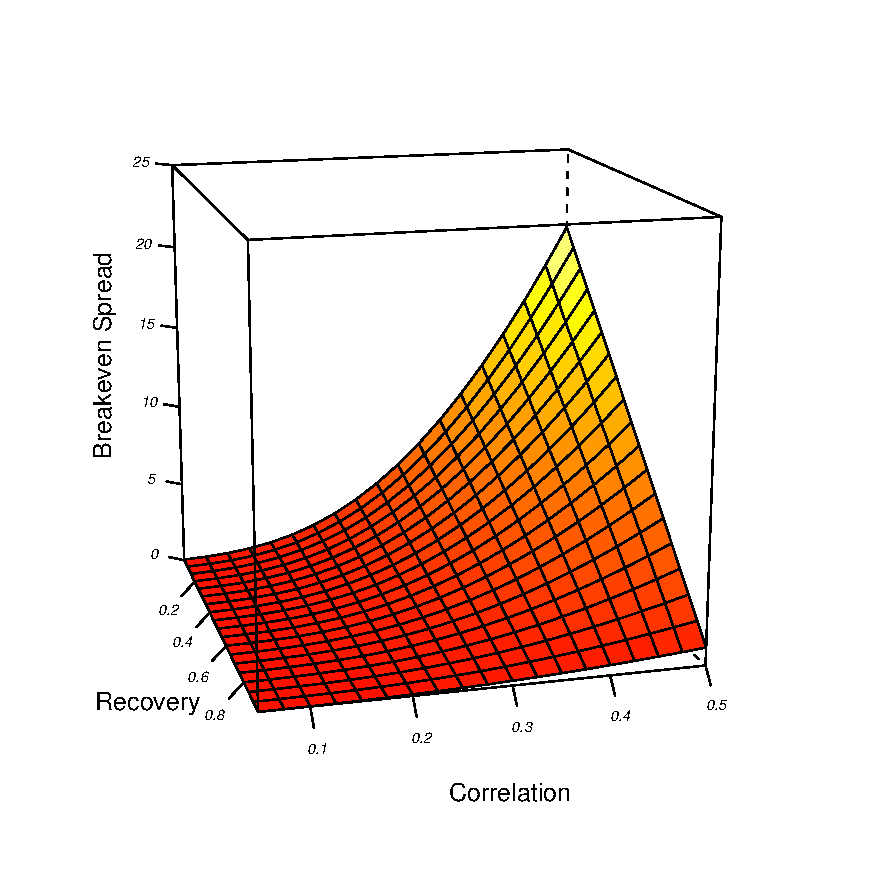
\includegraphics{pictures/BasketSpreads_Aug24.pdf}}}
{\scalebox{0.5}{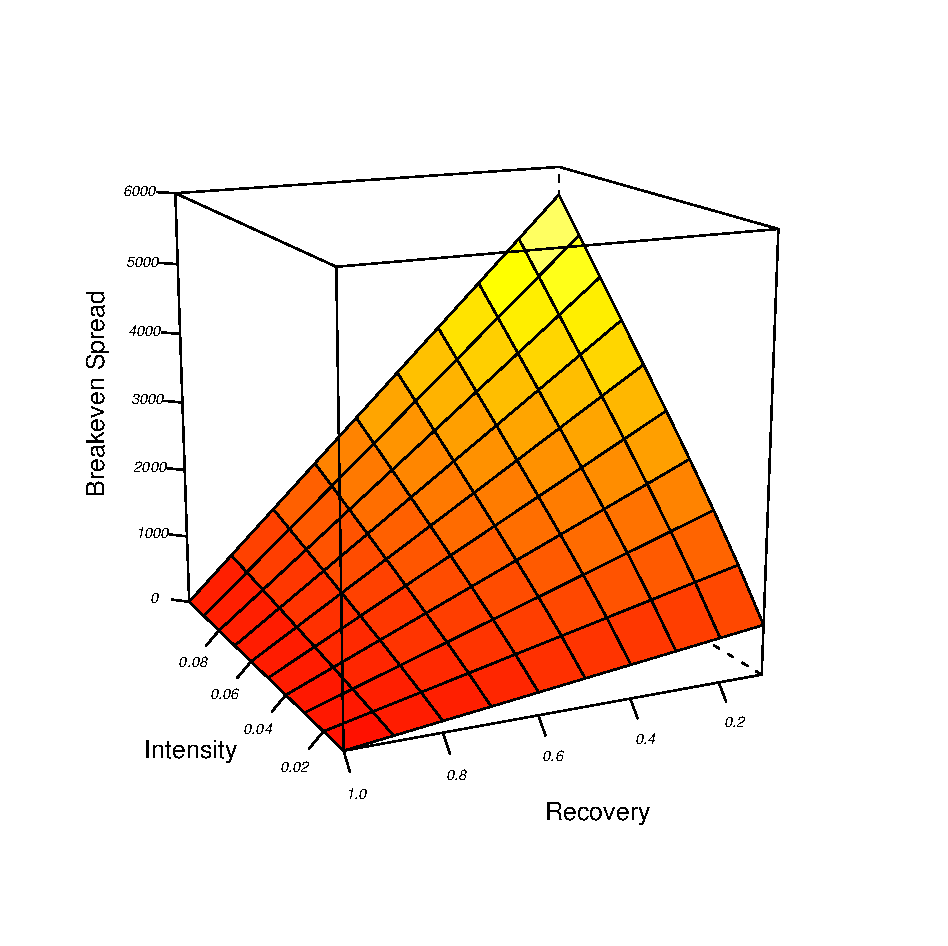
\includegraphics{pictures/BasketSpreadsIntensityRec_Aug27.pdf}}}
\caption{\label{fig:BasketSpreads}NTD Spreads for a basket of 10 entities considering the 6th to default with varying recovery rate, intensity and correlation}
\end{figure}

\begin{figure}
{\scalebox{0.5}{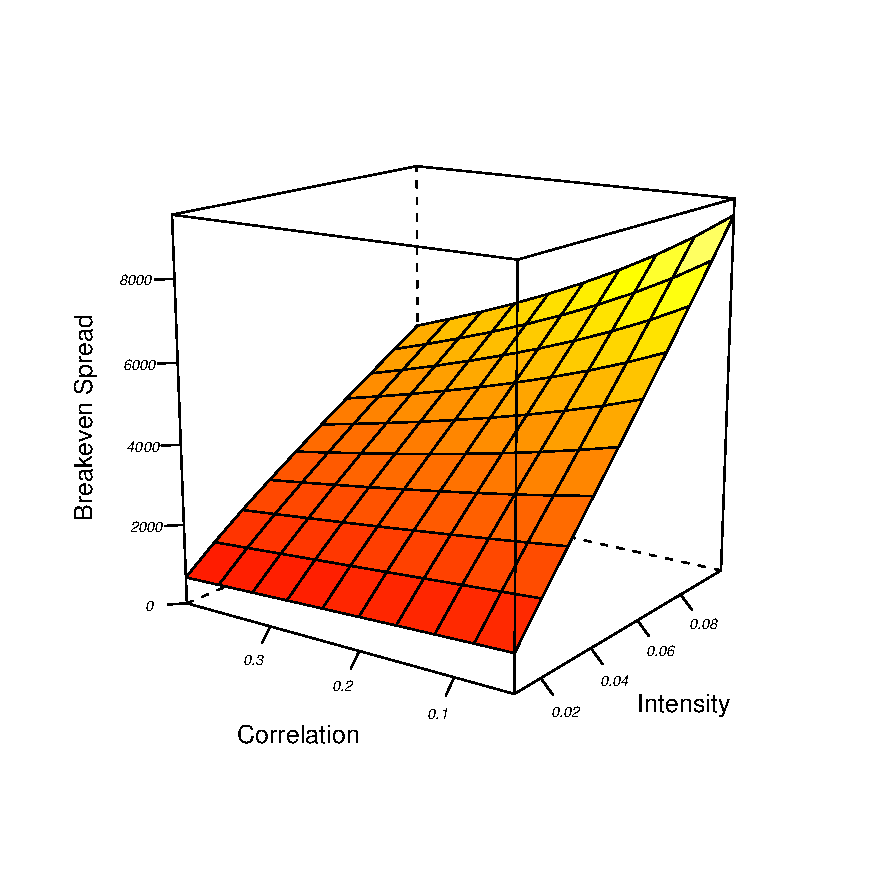
\includegraphics{pictures/BasketSpreadsFTDIntensity_Aug25.pdf}}}
{\scalebox{0.5}{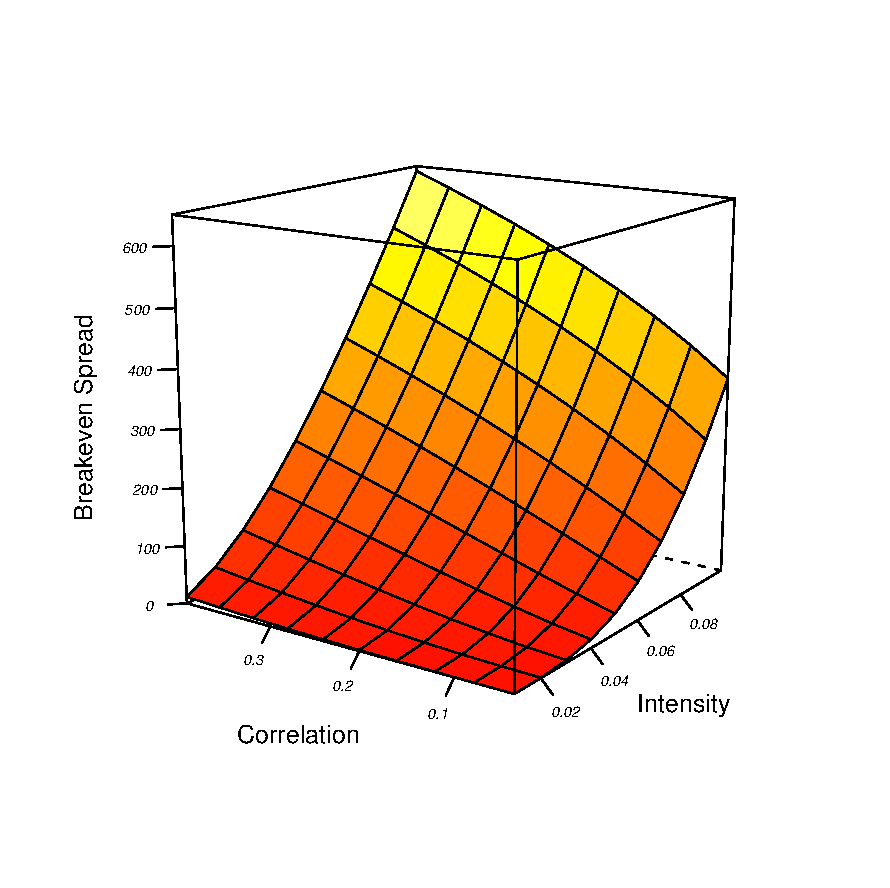
\includegraphics{pictures/BasketSpreadsIntensity_Aug24.pdf}}}
\caption{\label{fig:IntensityBasketSpreads}A comparison of intensity for a basket of 10 entities considering the 1st to default (left) and the 6th to default (right) with varying correlation and default intensity}
\end{figure}


\subsection{The effects of default intensity}

In figure~\ref{fig:IntensityBasketSpreads} we compare the intensity of a First to default (NTD, seniority = 1) against that of a 6th to default basket swap with varying correlation.  As the correlation increases we see the spreads increase for the higher default $n$ in an NTD whilst decreasing for the FTD.  Why is this so?  If our basket were perfectly correlated defaults would occur simultaneously and so the NTD spreads would be the same for all $n$.  For a much lower correlation, close to 0, the spreads decrease as it is highly unlikely for the defaults to cluster.  This becomes more pronounced as the default intensity itself increases, as we can see. The rate of increase is decreasing for low $n$ (figure~\ref{fig:IntensityBasketSpreads},left) and increasing for higher $n$ (figure~\ref{fig:IntensityBasketSpreads},right). This result extends Table 1 of \cite{hw2004} which shows this for 3 intensity points.  For very low intensities we see that increasing correlation lowers the spreads very slightly for FTDs and raises them for NTDs.  As intensities themselves increase correlation becomes more important so the correct intensity must be chosen within basket swap modeling. \cite{hw2004} looks at the dispersion of intensities relative to an average of 0.01 and finds that convexity is increased raising the prospect of one default and lowering the prospect of multiple defaults.


\section{CDO simulations}\label{sec:cdo_exp}

\subsection{Gaussian vs. Student-t Copula}\index{Copula Functions! Comparision}

Firstly, we present our spreads achieved for CDO pricing and compare a normal against a student-t distribution. \cite{Eli2006} states that the normal gaussian cannot fit prices of different CDO tranches with a single $\rho$ though the Student-t copula corrects this but does require more computation. In Figure~\ref{fig:tranchespreads} we compare spreads computed using Gaussian and Student-t distributions with 4 degrees of freedom. We see that across correlations the Student-t distribution is slightly higher for the equity tranche and slightly lower for the remaining tranches. A Student-t distribution should allow for more extreme events and so we should see more defaults in the equity tranche and fewer in the senior tranches, accounting for these differences.  Note that this spread structure of figure~\ref{fig:tranchespreads}, using our R CDO Pricing routine (see~\ref{sec:cdo_price}), is in line with published results \cite{hw2004,bv2005}. Variation of the degress of freedom of the $t$-distribution would be another avenue for interesting results.


\begin{figure}
{\scalebox{0.45}{\includegraphics{pictures/TrancheSpreads.pdf}}}
{\scalebox{0.45}{\includegraphics{pictures/TrancheSpreads_studentt.pdf}}}
\caption{\label{fig:tranchespreads}Tranche Spreads across Correlations for Equity, Mezzanine and Senior Tranches of a CDO}
\end{figure}

We examine the exposure to correlation risk \cite{Gib2004} wherein it is noted that tranches have sensitivity to the business cycle given that tranches have a dependency on default correlation and this may therefore be considered to be a business cycle risk.  \cite{Gib2004} refers to this as "most insightful".

\begin{figure}
{\scalebox{0.5}{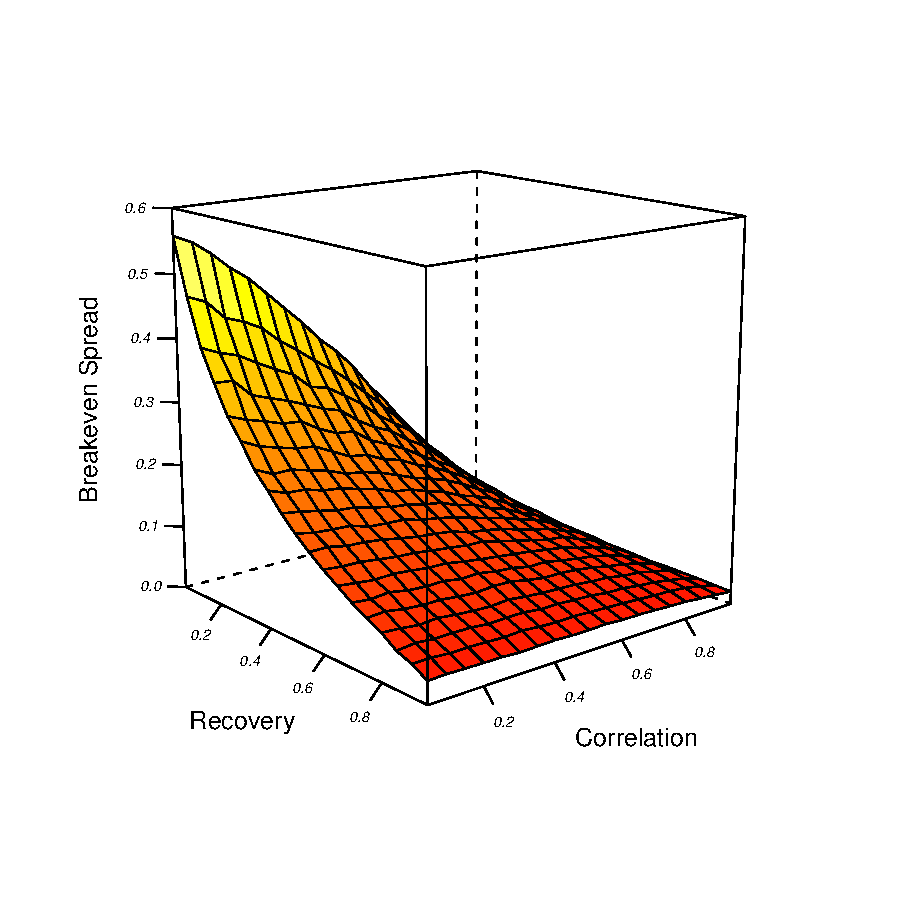
\includegraphics{pictures/CDOsim_June30_RecCor_EqTranche.pdf}}}
{\scalebox{0.5}{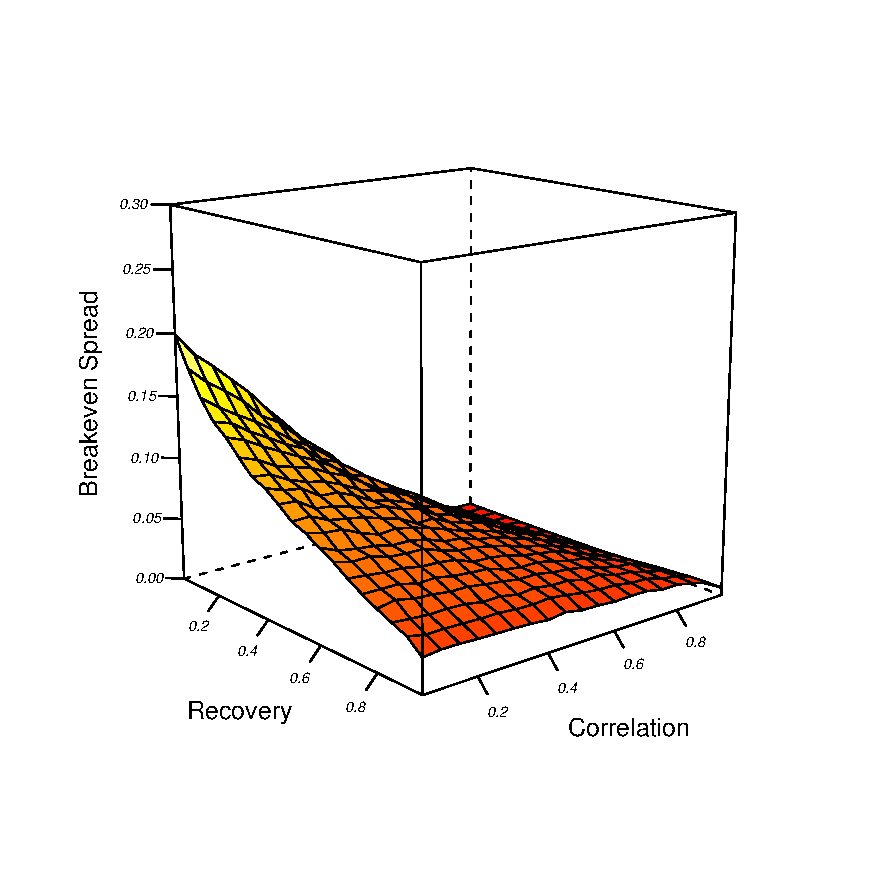
\includegraphics{pictures/CDOsim_Aug18_RecCor_MezzTranche.pdf}}}
{\scalebox{0.5}{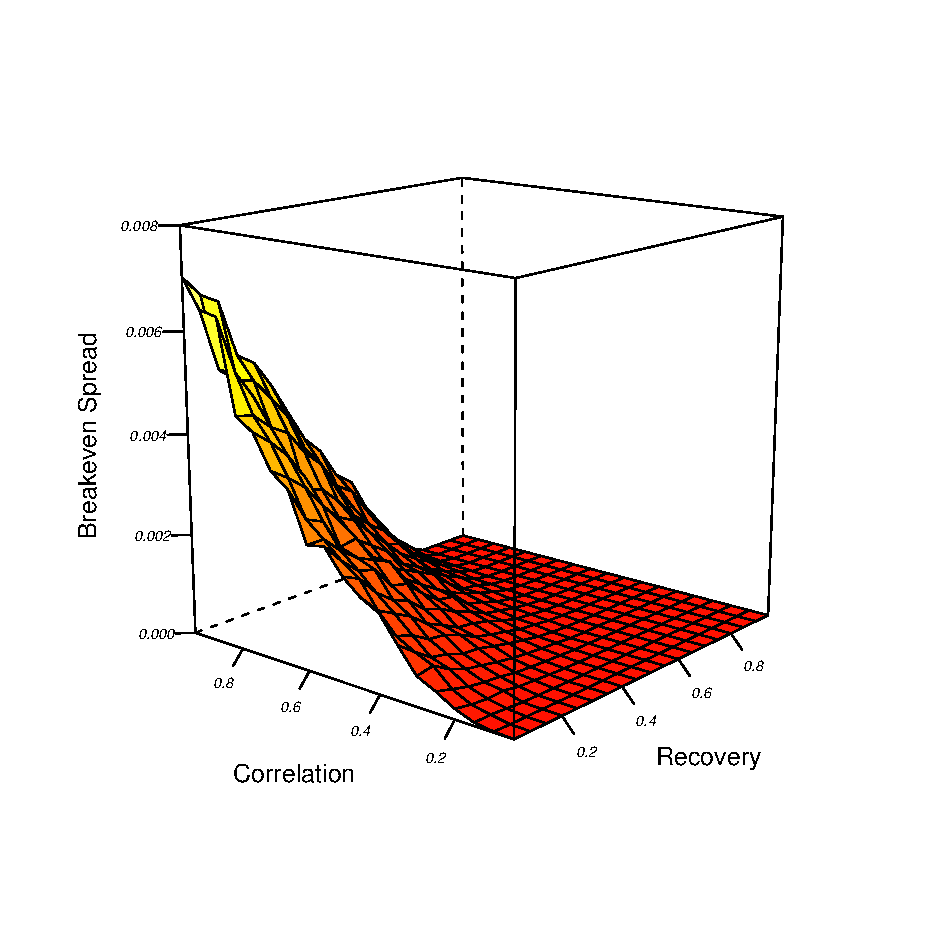
\includegraphics{pictures/CDOsim_Aug28_RecCor_SupSenTranche22_100.pdf}}}
\caption{\label{fig:CorRecSurface}Equity, Mezzanine and Senior Tranche for CDO, simulations varying recovery rate and correlation (Spreads:bps)}
\end{figure}

\subsection{Tranche Comparison}

In figure~\ref{fig:CorRecSurface} we present simulations for the equity (0-3\%, top left), mezzanine (6-9\%, top right) and super senior tranche (12-22\%, bottom) of a CDO generating the breakeven spread across recovery rates and correlation defaults. Mezzanine spreads are lower that those of the Equity tranche with the Senior  and Super Senior tranches being even lower.

 We see that the the higher correlation the higher the default probabilities and a decrease in premium which is monotonic on default correlation.  Clearly for the senior tranche the breakeven spreads are much lower but we can still see that the higher the recovery rate and the lower the correlation the higher the spread. Junior Mezzanine (3-6\%) and senior (9-12\%) tranches exhibited the same behaviour as mezzanine and super senior tranches but with slightly higher and lower, respectively, spreads. Figure~\ref{fig:CorRecSurface} shows that the correlation spread relationship for equity and mezzanine tranches is inverted for senior tranches. In the figure we highlight a super senior tranche (bottom) of 12-22\% which exhibits the same surface as a senior tranche but with lower spreads.  Why do we see this inversion across tranches? The reason for this is that the senior tranche is only likely to experience default when there are multiple defaults (high correlation) and the equity tranche (first loss tranche) is affected by any defaults. Even then we have seen that the spreads are small and any correlation must be high for the senior tranches.

We also see a slight saddle from high correlation / low recovery rate to high recovery rate/ low correlation in Equity and Mezzanine tranches, the effect being more pronounced in the latter. This is most probably due to the mezzanine tranches affected by second/third losses.

\begin{figure}
\centerline{\scalebox{0.5}{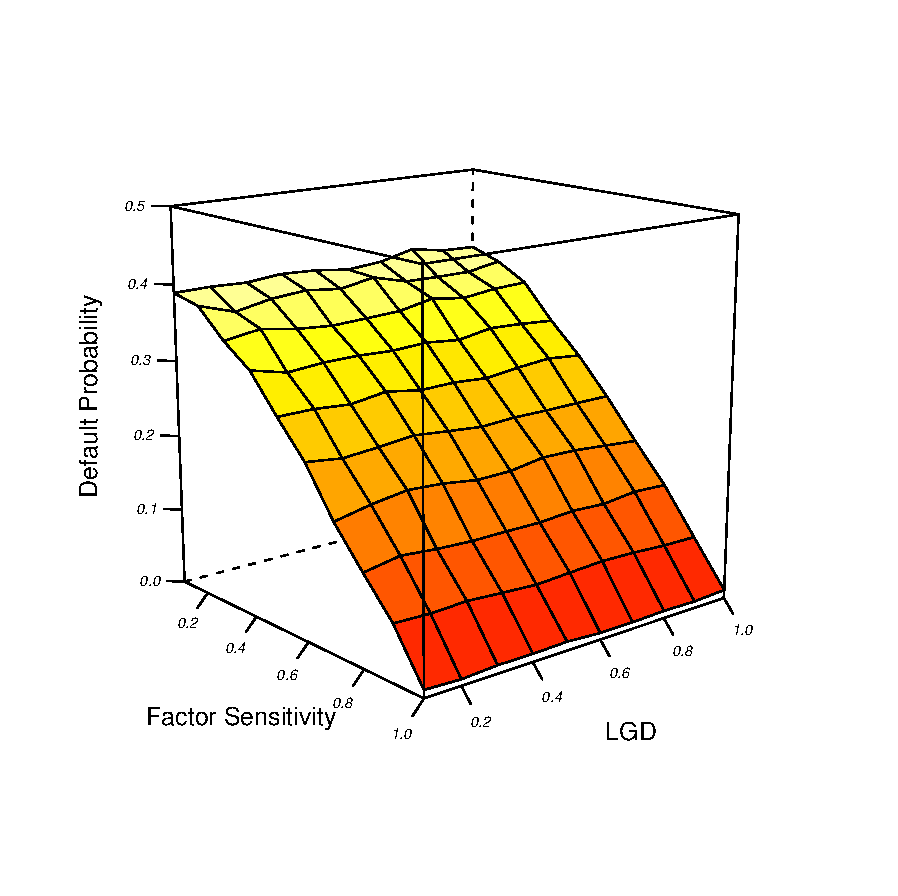
\includegraphics{pictures/EqTranche.pdf}}}
\centerline{\scalebox{0.5}{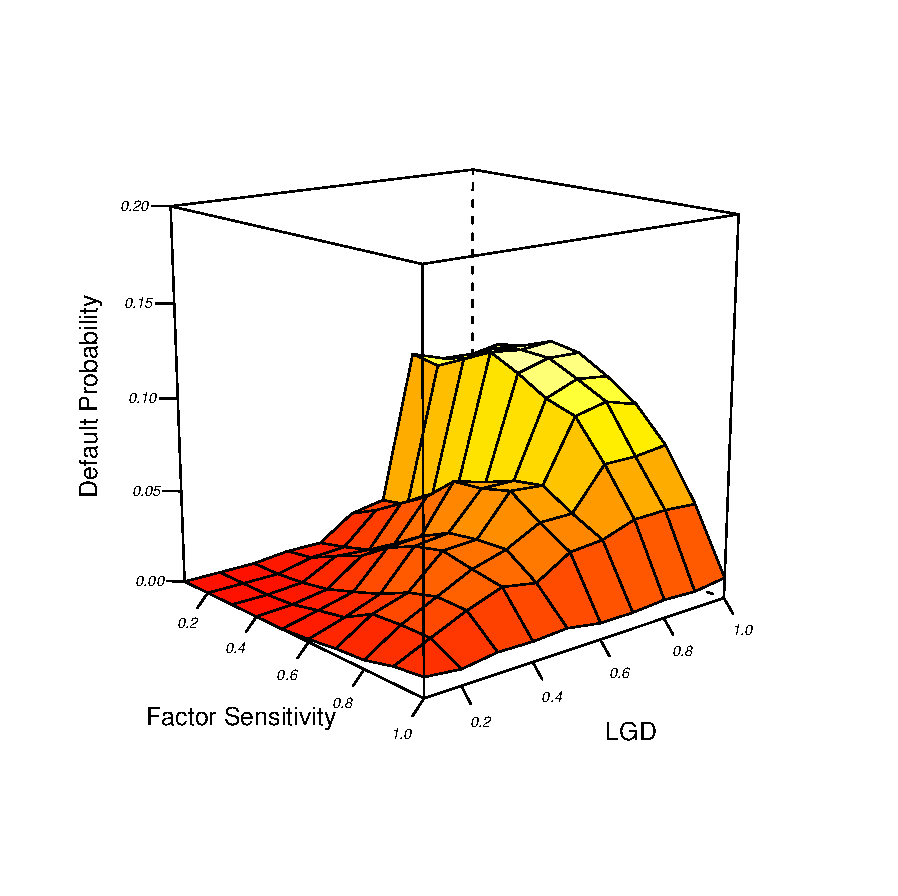
\includegraphics{pictures/MezzTranche.pdf}}}
\centerline{\scalebox{0.5}{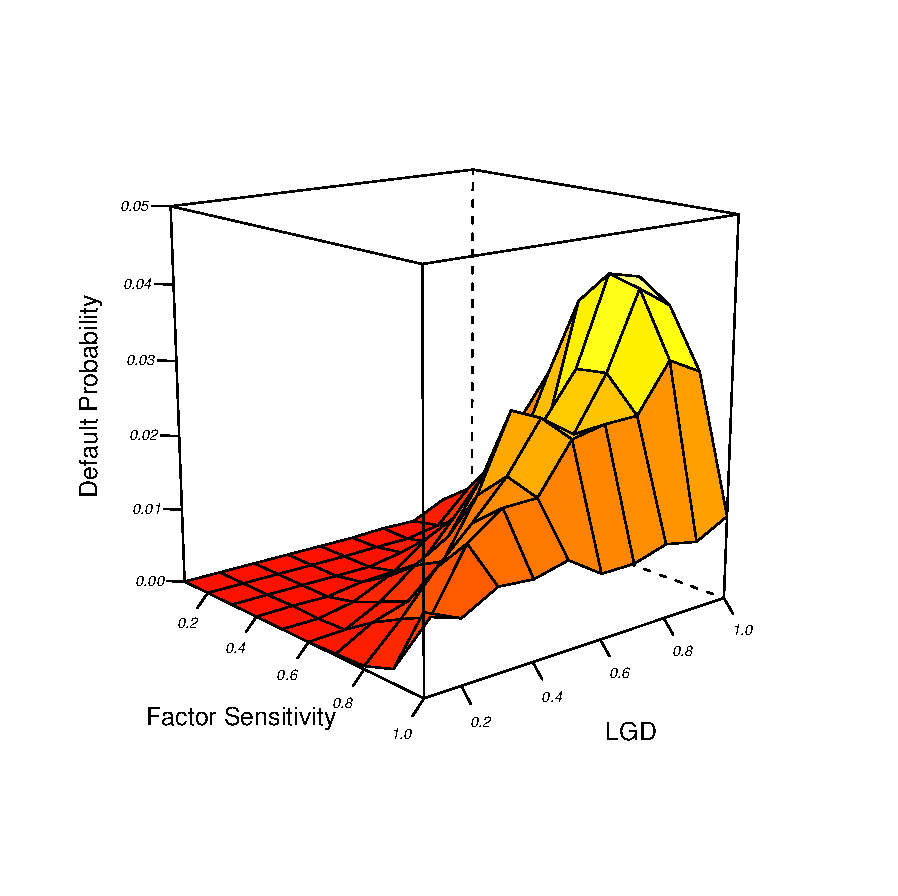
\includegraphics{pictures/SenTranche.pdf}}}
\caption{\label{fig:Unknown copula density}Equity,Mezzanine and Senior Tranche across LGDs and Factor Sensitivities (Spreads:bps)}
\end{figure}

\subsection{Factor Sensitivity}

In Figure~\ref{fig:Unknown copula density} we show results for simulations of a portfolio of 50 assets running 10000 simulations for each point. For the equity tranche we see the probability of default decrease as the factor sensitivity increase for all possible LGDs. This factor sensitivity to systemic risk suggests that the economy is {\em good} and so default probability will be low. Any increases in factor sensitivity (correlation) suggest there is more chance of no default occurring. As the LGD increases the default probability increases sharply around 0.7 but at a decreasing rate for increasing factor sensitivity.

 In the mezzanine tranche the probability of default increases slowly then decreases as LGDs increase and for the senior tranche the probability of default sharply increases then sharply decreases in increasing LDGs.  Factor sensitivity and LGD must be high for there to be a non-negligible default probability within the senior tranches. High correlation within the senior tranche implies that there is a chance of multiple defaults and we see this for figure~\ref{fig:Unknown copula density} (bottom).  The generation of these default probabilities replicates how ratings agencies use default probabilities to assign ratings to CDO tranches.




\section{Base Correlation - Why use this?}\index{Base Correlation}


In Figure~\ref{fig:tranchespreads} we see that for the Mezzanine and Sub-Senior tranches there are two correlations for a particular spread.  This means that standard implied correlation generates two solutions and motivates the requirement for base correlation. A Base Correlation skew is shown in figure~\ref{fig:impCorr}.
We note that data obtained for this work for the CDX and iTraxx indices shows that spreads have significantly increased since the publication of \cite{KL2004,hw2004}.


